\documentclass[tikz,border=10pt]{standalone}
\usepackage{tikz-3dplot}
\usepackage{amsmath, amssymb}
\usetikzlibrary{arrows.meta, positioning, calc, decorations.pathreplacing, 3d}
\usetikzlibrary{matrix, fit, backgrounds, shapes}
\usetikzlibrary{angles,quotes}

\usepackage[T1]{fontenc}
\usepackage[utf8]{inputenc}
\usepackage{newpxtext,newpxmath}
\usepackage{sectsty}

\begin{document}
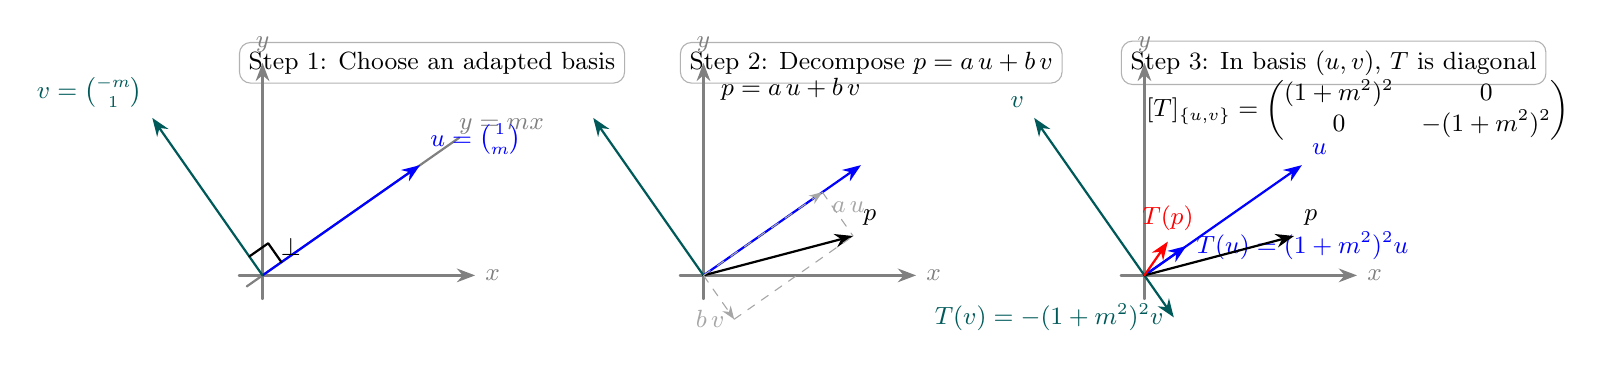
\begin{tikzpicture}[scale=2.0, >=Stealth, line cap=round, line join=round]
	
	%======================
	% PARAMETERS (edit here)
	%======================
	\def\m{0.7}          % slope m (axis y=mx)
	\def\vx{0.95}        % sample vector p=(vx,vy)
	\def\vy{0.25}
	
	%======================
	% COMPUTATIONS
	%======================
	% u=(1,m), v=(-m,1)
	\pgfmathsetmacro{\ux}{1}
	\pgfmathsetmacro{\uy}{\m}
	\pgfmathsetmacro{\vxB}{-\m}
	\pgfmathsetmacro{\vyB}{1}
	
	% scale s=(1+m^2)^2 for T (since T=(1+m^2)B and Bu=(1+m^2)u, Bv=-(1+m^2)v)
	\pgfmathsetmacro{\s}{(1+(\m)^2)^2}
	
	% Decompose p into p = a u + b v (solve [u v][a b]^T = p)
	% Matrix [u v] = [[1, -m],[m,1]], det = 1+m^2
	\pgfmathsetmacro{\den}{1+(\m)^2}
	\pgfmathsetmacro{\aa}{(\vx + \m*\vy)/\den}
	\pgfmathsetmacro{\bb}{(-\m*\vx + \vy)/\den}
	
	% Images under T in the (u,v) basis:
	% T(u)= s u,  T(v)= -s v, so T(p)= a s u + b (-s) v = s(a u - b v)
	\pgfmathsetmacro{\Tx}{\s*(\aa*\ux - \bb*\vxB)}  % careful: v basis vector is (-m,1)
	\pgfmathsetmacro{\Ty}{\s*(\aa*\uy - \bb*\vyB)}
	
	% Also show T(u), T(v)
	\pgfmathsetmacro{\Tux}{\s*\ux}
	\pgfmathsetmacro{\Tuy}{\s*\uy}
	\pgfmathsetmacro{\Tvx}{-\s*\vxB}
	\pgfmathsetmacro{\Tvy}{-\s*\vyB}
	
	%======================
	% STYLES
	%======================
	\tikzset{
		axis/.style={thick, gray},
		vecu/.style={thick, blue},
		vecv/.style={thick, teal!70!black},
		vecp/.style={thick, black},
		vect/.style={thick, red},
		dashedhelp/.style={dashed, gray!70},
		box/.style={rounded corners, draw=gray!60}
	}
	
	%======================
	% PANEL 1: Choose a basis (u,v)
	%======================
	\begin{scope}[shift={(0,0)}]
		\node[box, anchor=west] at (-0.15,1.35) {\small Step 1: Choose an adapted basis};
		
		% axes
		\draw[axis,->] (-0.15,0) -- (1.35,0) node[right] {\small $x$};
		\draw[axis,->] (0,-0.15) -- (0,1.35) node[above] {\small $y$};
		
		% axis line y=mx
		\draw[thick, gray] (-0.1,{-0.1*\m}) -- (1.25,{1.25*\m})
		node[pos=0.95, above right] {\small $y=mx$};
		
		% u and v basis vectors
		\draw[vecu,->] (0,0) -- (\ux,\uy) node[pos=1, above right] {\small $u=\binom{1}{m}$};
		\draw[vecv,->] (0,0) -- (\vxB,\vyB) node[pos=1, above left] {\small $v=\binom{-m}{1}$};
		
		% right-angle marker between axis and v at the origin (library-free)
		\pgfmathsetmacro{\rr}{0.12}
		% point along u from origin
		\coordinate (Uo) at ({\rr*\ux},{\rr*\uy});
		% point along v from origin
		\coordinate (Vo) at ({\rr*\vxB},{\rr*\vyB});
		\coordinate (Co) at ({\rr*\ux+\rr*\vxB},{\rr*\uy+\rr*\vyB});
		\draw[thick] (Uo) -- (Co) -- (Vo);
		\node at (0.18,0.18) {\small $\perp$};
		
	\end{scope}
	
	%======================
	% PANEL 2: Express a vector p in the basis (u,v)
	%======================
	\begin{scope}[shift={(2.8,0)}]
		\node[box, anchor=west] at (-0.15,1.35) {\small Step 2: Decompose $p=a\,u+b\,v$};
		
		% axes
		\draw[axis,->] (-0.15,0) -- (1.35,0) node[right] {\small $x$};
		\draw[axis,->] (0,-0.15) -- (0,1.35) node[above] {\small $y$};
		
		% u and v
		\draw[vecu,->] (0,0) -- (\ux,\uy);
		\draw[vecv,->] (0,0) -- (\vxB,\vyB);
		
		% p
		\coordinate (P) at (\vx,\vy);
		\draw[vecp,->] (0,0) -- (P) node[pos=1, above right] {\small $p$};
		
		% show a*u and b*v as a parallelogram sum
		\coordinate (AU) at ({\aa*\ux},{\aa*\uy});
		\coordinate (BV) at ({\bb*\vxB},{\bb*\vyB});
		\coordinate (AUplusBV) at ({\aa*\ux+\bb*\vxB},{\aa*\uy+\bb*\vyB});
		
		\draw[dashedhelp,->] (0,0) -- (AU) node[pos=1, below right] {\small $a\,u$};
		\draw[dashedhelp,->] (0,0) -- (BV) node[pos=1, left] {\small $b\,v$};
		
		\draw[dashedhelp] (AU) -- (AUplusBV);
		\draw[dashedhelp] (BV) -- (AUplusBV);
		
		% annotate equality
		\node[anchor=west] at (0.05,1.18) {\small $p=a\,u+b\,v$};
		
	\end{scope}
	
	%======================
	% PANEL 3: Action becomes diagonal in (u,v)
	%======================
	\begin{scope}[shift={(5.6,0)}]
		\node[box, anchor=west] at (-0.15,1.35) {\small Step 3: In basis $(u,v)$, $T$ is diagonal};
		
		% axes
		\draw[axis,->] (-0.15,0) -- (1.35,0) node[right] {\small $x$};
		\draw[axis,->] (0,-0.15) -- (0,1.35) node[above] {\small $y$};
		
		% Draw u and v directions (same)
		\draw[vecu,->] (0,0) -- (\ux,\uy) node[pos=1, above right] {\small $u$};
		\draw[vecv,->] (0,0) -- (\vxB,\vyB) node[pos=1, above left] {\small $v$};
		
		% show T(u)=s u and T(v)=-s v (scaled arrows; shorten visually with a factor)
		% For drawing, use a display scale factor to keep arrows on the page:
		\pgfmathsetmacro{\disp}{0.12} % purely visual
		\draw[vecu,->] (0,0) -- ({\disp*\Tux},{\disp*\Tuy})
		node[pos=1, right] {\small $T(u)= (1+m^2)^2u$};
		\draw[vecv,->] (0,0) -- ({\disp*\Tvx},{\disp*\Tvy})
		node[pos=1, left] {\small $T(v)= -(1+m^2)^2v$};
		
		% p and T(p) (again, visually scaled)
		\coordinate (P2) at (\vx,\vy);
		\coordinate (TP) at ({\disp*\Tx},{\disp*\Ty});
		
		\draw[vecp,->] (0,0) -- (P2) node[pos=1, above right] {\small $p$};
		\draw[vect,->] (0,0) -- (TP) node[pos=1, above] {\small $T(p)$};
		
		% text: diagonal matrix in basis B={u,v}
		\node[anchor=west] at (-0.05,1.05) {\small $
			[T]_{\{u,v\}}=
			\begin{pmatrix}
				(1+m^2)^2 & 0\\
				0 & -(1+m^2)^2
			\end{pmatrix}$};
		
	\end{scope}
	
\end{tikzpicture}

	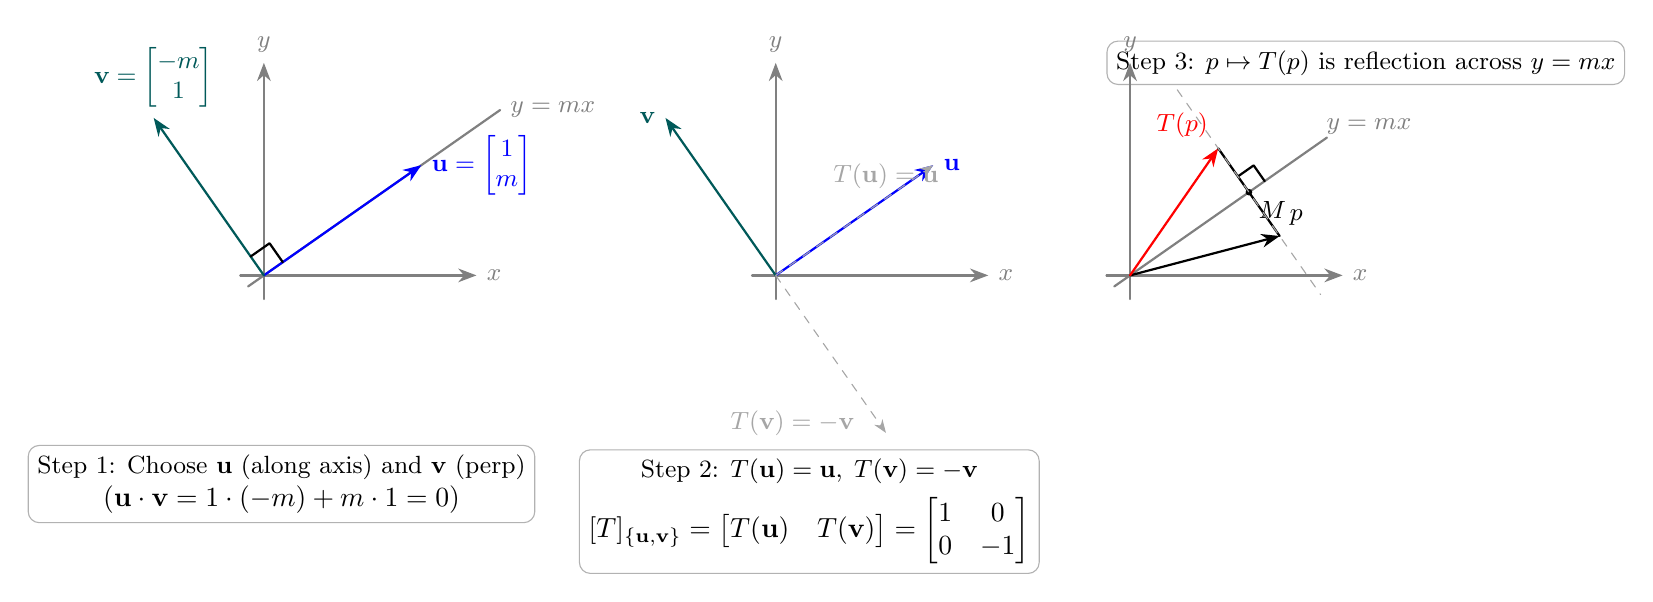
\begin{tikzpicture}[scale=2.0, >=Stealth, line cap=round, line join=round]
	
	%======================
	% PARAMETERS (edit here)
	%======================
	\def\m{0.7}          % slope m (axis y=mx)
	\def\px{0.95}        % sample vector p=(px,py)
	\def\py{0.25}
	
	%======================
	% COMPUTATIONS
	%======================
	% Reflection matrix A = 1/(1+m^2) [[1-m^2,2m],[2m,m^2-1]]
	\pgfmathsetmacro{\den}{1+(\m)^2}
	\pgfmathsetmacro{\a}{(1-(\m)^2)/\den}
	\pgfmathsetmacro{\b}{(2*\m)/\den}
	\pgfmathsetmacro{\c}{(2*\m)/\den}
	\pgfmathsetmacro{\d}{((\m)^2-1)/\den}
	
	% u=(1,m), v=(-m,1)
	\pgfmathsetmacro{\ux}{1}
	\pgfmathsetmacro{\uy}{\m}
	\pgfmathsetmacro{\vxB}{-\m}
	\pgfmathsetmacro{\vyB}{1}
	
	% Image Tp = A p
	\pgfmathsetmacro{\Tx}{\a*\px + \b*\py}
	\pgfmathsetmacro{\Ty}{\c*\px + \d*\py}
	
	% Midpoint M=(p+Tp)/2 lies on the axis y=mx; segment p--Tp is perpendicular to axis
	\pgfmathsetmacro{\mx}{(\px+\Tx)/2}
	\pgfmathsetmacro{\my}{(\py+\Ty)/2}
	
	% Styles
	\tikzset{
		axis/.style={thick, gray},
		vecu/.style={thick, blue},
		vecv/.style={thick, teal!70!black},
		vecp/.style={thick, black},
		vect/.style={thick, red},
		dashedhelp/.style={dashed, gray!70},
		box/.style={rounded corners, draw=gray!60, fill=white}
	}
	
	%======================
	% PANEL 1: Choose basis (u,v)
	%======================
	\begin{scope}[shift={(0,0)}]
		\node[box, anchor=west, align=center] at (-1.5,-1.325) {\small Step 1: Choose $\textbf{u}$ (along axis) and $\textbf{v}$ (perp)\\ ($\textbf{u}\cdot\textbf{v}=1\cdot(-m)+m\cdot 1=0$)};
		
		\draw[axis,->] (-0.15,0) -- (1.35,0) node[right] {\small $x$};
		\draw[axis,->] (0,-0.15) -- (0,1.35) node[above] {\small $y$};
		
		\draw[thick, gray] (-0.1,{-0.1*\m}) -- (1.5,{1.5*\m})
		node[pos=1, right] {\small $y=mx$};
		
		\draw[vecu,->] (0,0) -- (\ux,\uy) node[pos=1, right] {\small $\textbf{u}=\begin{bmatrix}
				1 \\ m
			\end{bmatrix}$};
		\draw[vecv,->] (0,0) -- (\vxB,\vyB) node[pos=1, above] {\small $\textbf{v}=\begin{bmatrix}
				-m \\ 1
			\end{bmatrix}$};
		
		% right-angle marker at origin between u and v (library-free)
		\pgfmathsetmacro{\rr}{0.12}
		\coordinate (Uo) at ({\rr*\ux},{\rr*\uy});
		\coordinate (Vo) at ({\rr*\vxB},{\rr*\vyB});
		\coordinate (Co) at ({\rr*\ux+\rr*\vxB},{\rr*\uy+\rr*\vyB});
		\draw[thick] (Uo) -- (Co) -- (Vo);
	\end{scope}
	
	%======================
	% PANEL 2: In this basis, the matrix is diagonal
	%======================
	\begin{scope}[shift={(3.25,0)}]
		\node[box, anchor=west, align=center] at (-1.25,-1.5) {\small Step 2: $T(\textbf{u})=\textbf{u},\;T(\textbf{v})=-\textbf{v}$\\ [4pt] $[T]_{\{\textbf{u},\textbf{v}\}}=\begin{bmatrix}
				T(\textbf{u}) & T(\textbf{v})
			\end{bmatrix}=\begin{bmatrix}
			1 & 0 \\ 0 & -1
		\end{bmatrix}$};
		
		\draw[axis,->] (-0.15,0) -- (1.35,0) node[right] {\small $x$};
		\draw[axis,->] (0,-0.15) -- (0,1.35) node[above] {\small $y$};
		
		\draw[vecu,->] (0,0) -- (\ux,\uy) node[pos=1, right] {\small $\textbf{u}$};
		\draw[vecv,->] (0,0) -- (\vxB,\vyB) node[pos=1, left] {\small $\textbf{v}$};
		
		% show images: u stays, v flips
		\draw[dashedhelp,->] (0,0) -- (\ux,\uy) node[pos=0.7, above] {\small $T(\textbf{u})=\textbf{u}$};
		\draw[dashedhelp,->] (0,0) -- ({-\vxB},{-\vyB}) node[pos=0.8, below left] {\small $T(\textbf{v})=-\textbf{v}$};
	\end{scope}
	
	%======================
	% PANEL 3: Reflect a sample vector p to Tp; show perpendicular to axis
	%======================
	\begin{scope}[shift={(5.5,0)}]
		\node[box, anchor=west] at (-0.15,1.35) {\small Step 3: $p\mapsto T(p)$ is reflection across $y=mx$};
		
		\draw[axis,->] (-0.15,0) -- (1.35,0) node[right] {\small $x$};
		\draw[axis,->] (0,-0.15) -- (0,1.35) node[above] {\small $y$};
		
		\draw[thick, gray] (-0.1,{-0.1*\m}) -- (1.25,{1.25*\m})
		node[pos=0.95, above right] {\small $y=mx$};
		
		\coordinate (P)  at (\px,\py);
		\coordinate (TP) at (\Tx,\Ty);
		\coordinate (M)  at (\mx,\my);
		
		\draw[vecp,->] (0,0) -- (P)  node[pos=1, above right] {\small $p$};
		\draw[vect,->] (0,0) -- (TP) node[pos=1, above left] {\small $T(p)$};
		
		% segment between p and T(p) is perpendicular to axis; midpoint lies on axis
		\draw[thick] (P) -- (TP);
		\fill (M) circle (0.6pt) node[below right] {\small $M$};
		
		% right-angle marker at M between axis direction (1,m) and segment direction (P-TP)
		% We mark right angle using axis direction u=(1,m) and normal direction n=(-m,1),
		% since the segment is parallel to n for a reflection.
		\pgfmathsetmacro{\s}{0.10}
		\coordinate (U1) at ({\mx+\s},{\my+\s*\m});        % along axis
		\coordinate (N1) at ({\mx-\s*\m},{\my+\s});        % along normal
		\coordinate (C1) at ({\mx+\s-\s*\m},{\my+\s*\m+\s});
		\draw[thick] (U1) -- (C1) -- (N1);
		
		% optional: draw the normal line through M (perpendicular to axis)
		\pgfmathsetmacro{\t}{0.65}
		\draw[dashedhelp] ({\mx-\t*\m},{\my+\t}) -- ({\mx+\t*\m},{\my-\t});
	\end{scope}
\end{tikzpicture}



	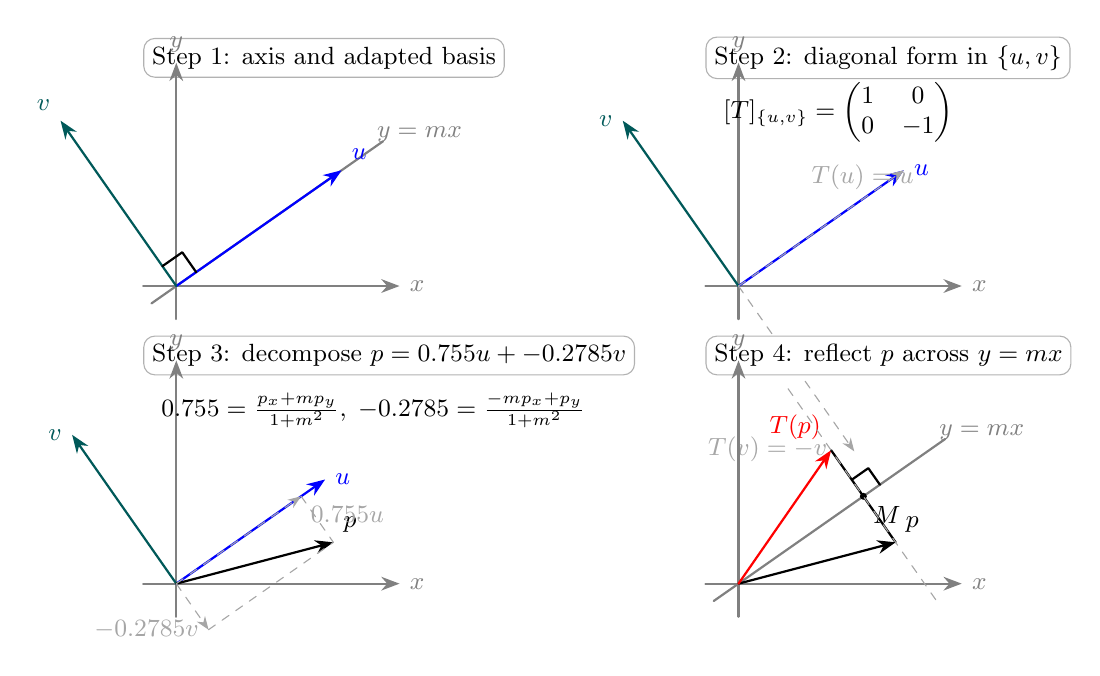
\begin{tikzpicture}[scale=2.1, >=Stealth, line cap=round, line join=round]
		
		%======================
		% PARAMETERS (edit here)
		%======================
		\def\m{0.7}          % slope m of the reflection axis y=mx
		\def\px{0.95}        % sample vector p = (px,py)
		\def\py{0.25}
		
		%======================
		% MATRIX A (reflection)
		%======================
		\pgfmathsetmacro{\den}{1+(\m)^2}
		\pgfmathsetmacro{\a}{(1-(\m)^2)/\den}
		\pgfmathsetmacro{\b}{(2*\m)/\den}
		\pgfmathsetmacro{\c}{(2*\m)/\den}
		\pgfmathsetmacro{\d}{((\m)^2-1)/\den}
		
		%======================
		% ADAPTED BASIS
		% u=(1,m) (along axis), v=(-m,1) (perp)
		%======================
		\pgfmathsetmacro{\ux}{1}
		\pgfmathsetmacro{\uy}{\m}
		\pgfmathsetmacro{\vxB}{-\m}
		\pgfmathsetmacro{\vyB}{1}
		
		%======================
		% IMAGE Tp = A p
		%======================
		\pgfmathsetmacro{\Tx}{\a*\px + \b*\py}
		\pgfmathsetmacro{\Ty}{\c*\px + \d*\py}
		
		% Midpoint M=(p+Tp)/2 lies on axis; segment p--Tp is perpendicular to axis
		\pgfmathsetmacro{\mx}{(\px+\Tx)/2}
		\pgfmathsetmacro{\my}{(\py+\Ty)/2}
		
		%======================
		% Decompose p = alpha u + beta v
		% [u v] = [[1,-m],[m,1]], det = 1+m^2
		%======================
		\pgfmathsetmacro{\alpha}{(\px + \m*\py)/\den}
		\pgfmathsetmacro{\beta}{(-\m*\px + \py)/\den}
		
		\coordinate (AU) at ({\alpha*\ux},{\alpha*\uy});
		\coordinate (BV) at ({\beta*\vxB},{\beta*\vyB});
		\coordinate (SUM) at ({\alpha*\ux+\beta*\vxB},{\alpha*\uy+\beta*\vyB});
		
		%======================
		% STYLES
		%======================
		\tikzset{
			axis/.style={thick, gray},
			box/.style={rounded corners, draw=gray!60, fill=white, inner sep=3pt},
			axline/.style={thick, gray},
			uvec/.style={thick, blue},
			vvec/.style={thick, teal!70!black},
			pvec/.style={thick, black},
			tvec/.style={thick, red},
			help/.style={dashed, gray!70}
		}
		
		% Utility: draw axes inside each panel
		\newcommand{\panelaxes}{
			\draw[axis,->] (-0.2,0) -- (1.35,0) node[right] {\small $x$};
			\draw[axis,->] (0,-0.2) -- (0,1.35) node[above] {\small $y$};
		}
		
		% Utility: right-angle marker at a point (X,Y) with directions u=(1,m) and n=(-m,1)
		\newcommand{\rightangleat}[3]{% (#1,#2)=point, #3=size
			\coordinate (RAU) at ({#1 + #3},{#2 + #3*\m});     % along axis
			\coordinate (RAN) at ({#1 - #3*\m},{#2 + #3});     % along normal
			\coordinate (RAC) at ({#1 + #3 - #3*\m},{#2 + #3*\m + #3});
			\draw[thick] (RAU) -- (RAC) -- (RAN);
		}
		
		%======================
		% 2x2 GRID OF PANELS
		% panel size ~ 1.6x1.6 (in TikZ coords)
		%======================
		
		%----------------------
		% Panel (1,1): Step 1
		%----------------------
		\begin{scope}[shift={(0,1.8)}]
			\node[box, anchor=west] at (-0.2,1.38) {\small Step 1: axis and adapted basis};
			
			\panelaxes
			
			\draw[axline] (-0.15,{-0.15*\m}) -- (1.25,{1.25*\m})
			node[pos=0.93, above right] {\small $y=mx$};
			
			\draw[uvec,->] (0,0) -- (\ux,\uy) node[pos=1, above right] {\small $u$};
			\draw[vvec,->] (0,0) -- (\vxB,\vyB) node[pos=1, above left] {\small $v$};
			
			% right-angle at origin between u and v
			\rightangleat{0}{0}{0.12}
		\end{scope}
		
		%----------------------
		% Panel (2,1): Step 2
		%----------------------
		\begin{scope}[shift={(3.4,1.8)}]
			\node[box, anchor=west] at (-0.2,1.38) {\small Step 2: diagonal form in $\{u,v\}$};
			
			\panelaxes
			
			\draw[uvec,->] (0,0) -- (\ux,\uy) node[pos=1, right] {\small $u$};
			\draw[vvec,->] (0,0) -- (\vxB,\vyB) node[pos=1, left] {\small $v$};
			
			% images: u fixed, v flipped
			\draw[help,->] (0,0) -- (\ux,\uy) node[pos=0.75, above] {\small $T(u)=u$};
			\draw[help,->] (0,0) -- ({-\vxB},{-\vyB}) node[pos=0.85, below left] {\small $T(v)=-v$};
			
			\node[anchor=west] at (-0.15,1.05) {\small $
				[T]_{\{u,v\}}=
				\begin{pmatrix}1&0\\0&-1\end{pmatrix}$};
		\end{scope}
		
		%----------------------
		% Panel (1,2): Step 3
		%----------------------
		\begin{scope}[shift={(0,0)}]
			\node[box, anchor=west] at (-0.2,1.38) {\small Step 3: decompose $p=\alpha u+\beta v$};
			
			\panelaxes
			
			% basis directions
			\draw[uvec,->] (0,0) -- ({0.9*\ux},{0.9*\uy}) node[pos=1, right] {\small $u$};
			\draw[vvec,->] (0,0) -- ({0.9*\vxB},{0.9*\vyB}) node[pos=1, left] {\small $v$};
			
			% p
			\coordinate (P) at (\px,\py);
			\draw[pvec,->] (0,0) -- (P) node[pos=1, above right] {\small $p$};
			
			% parallelogram
			\draw[help,->] (0,0) -- (AU) node[pos=1, below right] {\small $\alpha u$};
			\draw[help,->] (0,0) -- (BV) node[pos=1, left] {\small $\beta v$};
			\draw[help] (AU) -- (SUM);
			\draw[help] (BV) -- (SUM);
			
			\node[anchor=west] at (-0.15,1.05) {\small $
				\alpha=\frac{p_x+m p_y}{1+m^2},\;
				\beta=\frac{-m p_x+p_y}{1+m^2}$};
		\end{scope}
		
		%----------------------
		% Panel (2,2): Step 4
		%----------------------
		\begin{scope}[shift={(3.4,0)}]
			\node[box, anchor=west] at (-0.2,1.38) {\small Step 4: reflect $p$ across $y=mx$};
			
			\panelaxes
			
			% axis
			\draw[axline] (-0.15,{-0.15*\m}) -- (1.25,{1.25*\m})
			node[pos=0.93, above right] {\small $y=mx$};
			
			% p and T(p)
			\coordinate (P4) at (\px,\py);
			\coordinate (TP4) at (\Tx,\Ty);
			\coordinate (M) at (\mx,\my);
			
			\draw[pvec,->] (0,0) -- (P4) node[pos=1, above right] {\small $p$};
			\draw[tvec,->] (0,0) -- (TP4) node[pos=1, above left] {\small $T(p)$};
			
			% segment between p and T(p)
			\draw[thick] (P4) -- (TP4);
			
			% midpoint on axis
			\fill (M) circle (0.6pt) node[below right] {\small $M$};
			
			% draw normal through M (perpendicular to axis)
			\draw[help] ({\mx-0.65*\m},{\my+0.65}) -- ({\mx+0.65*\m},{\my-0.65});
			
			% right-angle marker at M
			\rightangleat{\mx}{\my}{0.10}
		\end{scope}
		
	\end{tikzpicture}

% Preamble:
% \usepackage{tikz}
% \usetikzlibrary{calc}

%\begin{center}
%	\begin{tikzpicture}[scale=2.05, >=Stealth, line cap=round, line join=round]
%		
%		%======================
%		% PARAMETERS (edit here)
%		%======================
%		\def\m{0.7}          % slope of reflection axis y=mx
%		\def\px{0.95}        % sample vector p=(px,py)
%		\def\py{0.25}
%		
%		%======================
%		% BASIC VECTORS
%		% u=(1,m), v=(-m,1)
%		%======================
%		\pgfmathsetmacro{\ux}{1}
%		\pgfmathsetmacro{\uy}{\m}
%		\pgfmathsetmacro{\vxB}{-\m}
%		\pgfmathsetmacro{\vyB}{1}
%		
%		%======================
%		% DECOMPOSITION p = alpha u + beta v
%		% [u v]=[[1,-m],[m,1]], det=1+m^2
%		% alpha=(px+m py)/(1+m^2), beta=(-m px+py)/(1+m^2)
%		%======================
%		\pgfmathsetmacro{\den}{1+(\m)^2}
%		\pgfmathsetmacro{\alpha}{(\px + \m*\py)/\den}
%		\pgfmathsetmacro{\beta}{(-\m*\px + \py)/\den}
%		
%		\coordinate (AU)  at ({\alpha*\ux},{\alpha*\uy});
%		\coordinate (BV)  at ({\beta*\vxB},{\beta*\vyB});
%		\coordinate (SUM) at ({\alpha*\ux+\beta*\vxB},{\alpha*\uy+\beta*\vyB});
%		
%		%======================
%		% REFLECTION WITHOUT "KNOWING A"
%		% In {u,v}-coordinates: (a,b) -> (a,-b)
%		% So T(p)= alpha u - beta v
%		%======================
%		\coordinate (TP) at ({\alpha*\ux-\beta*\vxB},{\alpha*\uy-\beta*\vyB});
%		
%		% Midpoint M between p and T(p) lies on the axis; segment p--T(p) ⟂ axis
%		\pgfmathsetmacro{\mx}{(\px + (\alpha*\ux-\beta*\vxB))/2}
%		\pgfmathsetmacro{\my}{(\py + (\alpha*\uy-\beta*\vyB))/2}
%		\coordinate (M) at (\mx,\my);
%		
%		%======================
%		% STYLES
%		%======================
%		\tikzset{
%			axis/.style={thick, gray},
%			box/.style={rounded corners, draw=gray!60, fill=white, inner sep=3pt},
%			axline/.style={thick, gray},
%			uvec/.style={thick, blue},
%			vvec/.style={thick, teal!70!black},
%			pvec/.style={thick, black},
%			tvec/.style={thick, red},
%			help/.style={dashed, gray!70},
%			mat/.style={font=\small}
%		}
%		
%		% Utility: axes in panel
%		\newcommand{\panelaxes}{
%			\draw[axis,->] (-0.2,0) -- (1.35,0) node[right] {\small $x$};
%			\draw[axis,->] (0,-0.2) -- (0,1.35) node[above] {\small $y$};
%		}
%		
%		% Utility: right-angle marker at (X,Y) using axis direction (1,m) and normal (-m,1)
%		\newcommand{\rightangleat}[3]{% X,Y,size
%			\coordinate (RAU) at ({#1 + #3},{#2 + #3*\m});     % along axis
%			\coordinate (RAN) at ({#1 - #3*\m},{#2 + #3});     % along normal
%			\coordinate (RAC) at ({#1 + #3 - #3*\m},{#2 + #3*\m + #3});
%			\draw[thick] (RAU) -- (RAC) -- (RAN);
%		}
%		
%		%======================
%		% 2x2 PANELS
%		%======================
%		
%		%----------------------
%		% Panel 1 (top-left): Choose adapted basis
%		%----------------------
%		\begin{scope}[shift={(0,1.8)}]
%			\node[box, anchor=west] at (-0.2,1.38) {\small Step 1: choose an axis/perp basis};
%			
%			\panelaxes
%			
%			\draw[axline] (-0.15,{-0.15*\m}) -- (1.25,{1.25*\m})
%			node[pos=0.93, above right] {\small $y=mx$};
%			
%			\draw[uvec,->] (0,0) -- (\ux,\uy) node[pos=1, above right] {\small $u=\binom{1}{m}$};
%			\draw[vvec,->] (0,0) -- (\vxB,\vyB) node[pos=1, above left]  {\small $v=\binom{-m}{1}$};
%			
%			% right angle marker at origin between axis-direction and perpendicular-direction
%			\rightangleat{0}{0}{0.12}
%			
%			\node[anchor=west, mat] at (-0.18,1.05) {$u\cdot v=0$ so $\{u,v\}$ is a basis.};
%		\end{scope}
%		
%		%----------------------
%		% Panel 2 (top-right): In this basis, reflection is simple
%		%----------------------
%		\begin{scope}[shift={(3.4,1.8)}]
%			\node[box, anchor=west] at (-0.2,1.38) {\small Step 2: define reflection in the new coordinates};
%			
%			\panelaxes
%			
%			\draw[uvec,->] (0,0) -- (\ux,\uy) node[pos=1, right] {\small $u$};
%			\draw[vvec,->] (0,0) -- (\vxB,\vyB) node[pos=1, left]  {\small $v$};
%			
%			% show the rule: keep u-component, flip v-component
%			\draw[help,->] (0,0) -- (\ux,\uy) node[pos=0.75, above] {\small $T(u)=u$};
%			\draw[help,->] (0,0) -- ({-\vxB},{-\vyB}) node[pos=0.80, below left] {\small $T(v)=-v$};
%			
%			\node[anchor=west, mat] at (-0.18,1.05) {$[T]_{\{u,v\}}=\begin{pmatrix}1&0\\0&-1\end{pmatrix}$.};
%		\end{scope}
%		
%		%----------------------
%		% Panel 3 (bottom-left): Decompose a vector p = αu + βv
%		%----------------------
%		\begin{scope}[shift={(0,0)}]
%			\node[box, anchor=west] at (-0.2,1.38) {\small Step 3: write $p=\alpha u+\beta v$};
%			
%			\panelaxes
%			
%			% draw u,v directions (short)
%			\draw[uvec,->] (0,0) -- ({0.9*\ux},{0.9*\uy}) node[pos=1, right] {\small $u$};
%			\draw[vvec,->] (0,0) -- ({0.9*\vxB},{0.9*\vyB}) node[pos=1, left]  {\small $v$};
%			
%			% p
%			\coordinate (P) at (\px,\py);
%			\draw[pvec,->] (0,0) -- (P) node[pos=1, above right] {\small $p$};
%			
%			% parallelogram
%			\draw[help,->] (0,0) -- (AU) node[pos=1, below right] {\small $\alpha u$};
%			\draw[help,->] (0,0) -- (BV) node[pos=1, left] {\small $\beta v$};
%			\draw[help] (AU) -- (SUM);
%			\draw[help] (BV) -- (SUM);
%			
%			\node[anchor=west, mat] at (-0.18,1.05) {$
%				\alpha=\frac{p_x+m p_y}{1+m^2},\quad
%				\beta=\frac{-m p_x+p_y}{1+m^2}$};
%		\end{scope}
%		
%		%----------------------
%		% Panel 4 (bottom-right): Apply reflection rule to get T(p)
%		%----------------------
%		\begin{scope}[shift={(3.4,0)}]
%			\node[box, anchor=west] at (-0.2,1.38) {\small Step 4: apply $(\alpha,\beta)\mapsto(\alpha,-\beta)$};
%			
%			\panelaxes
%			
%			% axis
%			\draw[axline] (-0.15,{-0.15*\m}) -- (1.25,{1.25*\m})
%			node[pos=0.93, above right] {\small $y=mx$};
%			
%			% p and T(p)
%			\coordinate (P4) at (\px,\py);
%			\draw[pvec,->] (0,0) -- (P4) node[pos=1, above right] {\small $p=\alpha u+\beta v$};
%			\draw[tvec,->] (0,0) -- (TP) node[pos=1, above left] {\small $T(p)=\alpha u-\beta v$};
%			
%			% segment and midpoint/right angle
%			\draw[thick] (P4) -- (TP);
%			\fill (M) circle (0.6pt) node[below right] {\small $M$};
%			
%			% normal through M (perp to axis)
%			\draw[help] ({\mx-0.65*\m},{\my+0.65}) -- ({\mx+0.65*\m},{\my-0.65});
%			
%			% right-angle marker at M
%			\rightangleat{\mx}{\my}{0.10}
%			
%			\node[anchor=west, mat] at (-0.18,1.05) {Then $T$ is reflection across $y=mx$.};
%		\end{scope}
%		
%	\end{tikzpicture}
%\end{center}

\end{document}